\section{Preliminary Definitions}
\label{sec:basicconcepts}

\subsection{eXecutable Domain-Specific Languages (xDSLs)}

A DSL is specified in terms of its abstract syntax, concrete syntax and semantics. There is a mapping between the concrete syntax and the semantics. Then, a DSL specification can be defined as triple $<AS, CS, Sem>$. In this paper we are focused on the definition of AS and Sem. Specially, in executable DSLs where the semantics is defined operationally. In that case, the semantics can be specified as a set of domain-specific actions (DSA) each of which is defined to a particular construct of the AS. 

\subsection{Families of xDSLs}

Although many of them are completely different and with independent domains; it is also true that we can find related DSLs with overlapping domains. Moreover, there are set of DSLs for which the domains can be hierarchically organized \cite[p. 60-61]{voelter:2013} (see Fig. \ref{fig:domains}). For instance, while DSLs for prototyping graphical user interfaces are usually independent from those who deal with data management, the DSL for expressing security policies presented in \cite{Lodderstedt:2002} overlaps the DSL for finite state machines presented in \cite{Hamann:2012}. This is because both of them use the notion of `constraints' that, in addition, is implemented in a common formalism (OCL in this case). In turn, a DSL for expressing state machines can be specialized for tackling with data refinement \cite{Schewe:2008}, consequently, the domain of the former can be viewed as a super-domain of the later. All the concepts in the state machines are contained in the data refinement DSLs. 

The aforementioned phenomenon is known in the literature under the notion of \textbf{families of DSLs} \cite{Zschaler:2010b}. A family is a set of DSLs that share some commonalities and that are distinguished each other by certain particularities. Certainly, commonalities among DSLs within a family of DSLs represent an opportunity for leveraging reuse during the language engineering process.

\begin{figure}
\centering
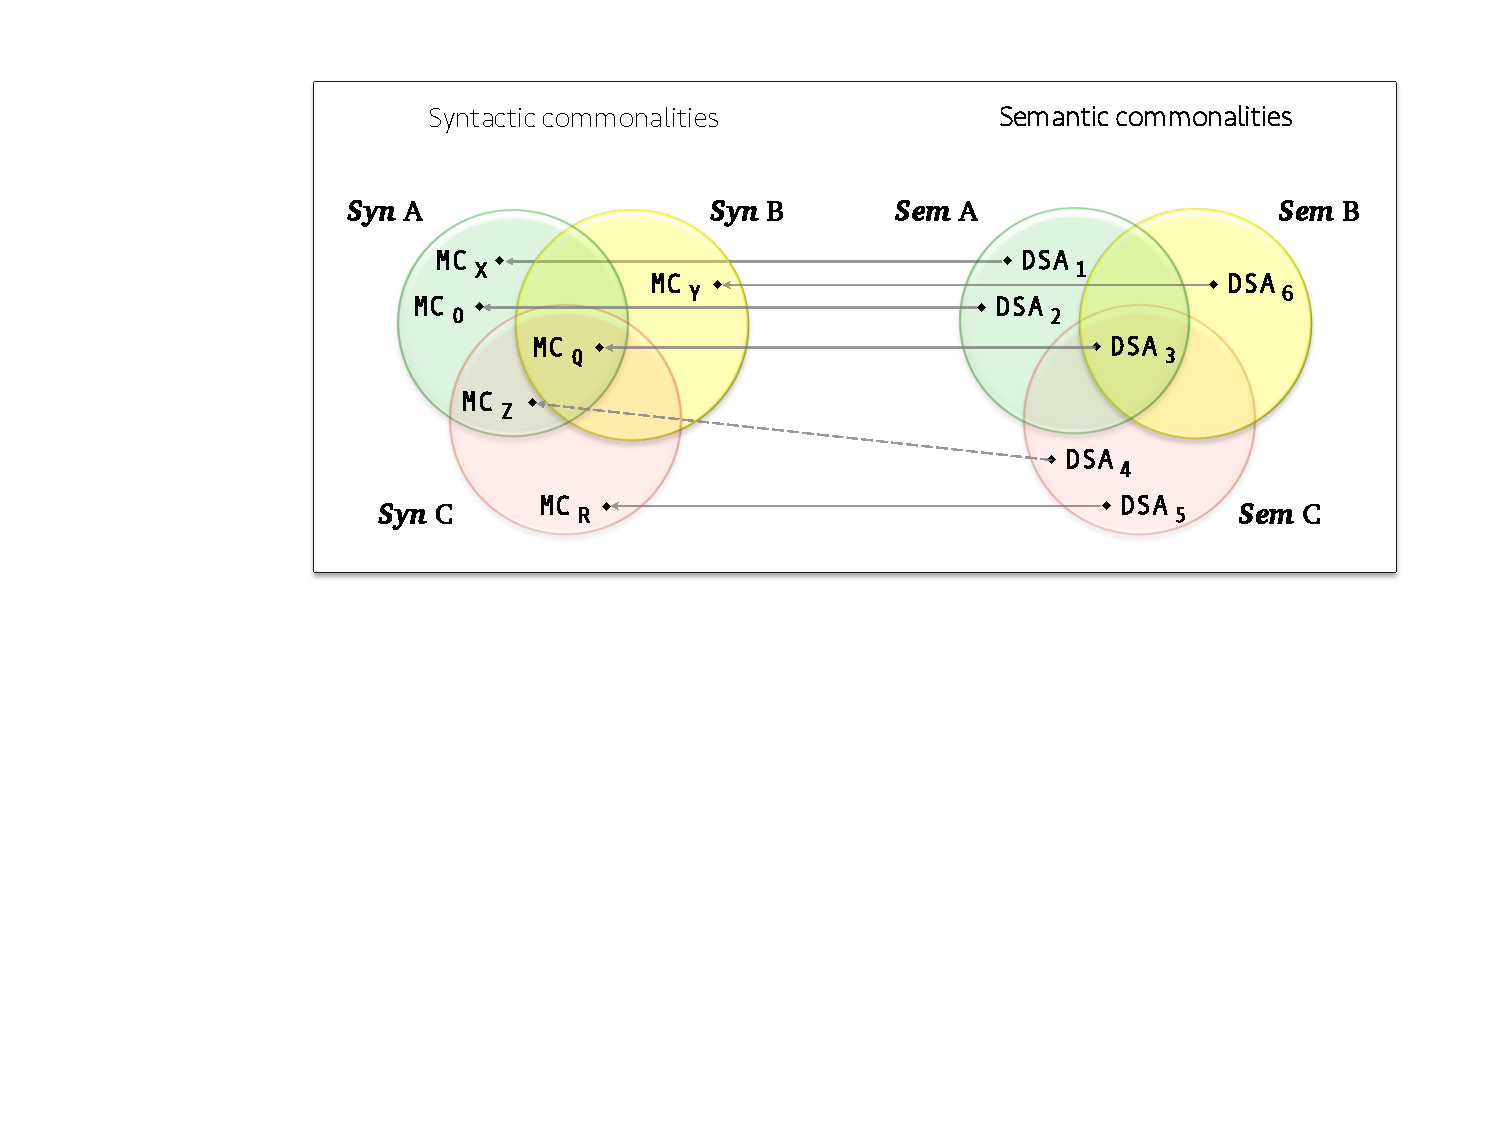
\includegraphics[width=1\linewidth]{images/domains-fig.pdf}
\caption{Different relationships between DSL domains}
\label{fig:domains}
\end{figure}

A family of xDSLs is a set of xDSLs that share some segments of their specification. 

\begin{mydef} A family of DSLs is language-centric, symbolized $\lambda(F)$, if and only if there exists a segment of the specification shared by all the family members.
\vspace{-1mm}
\begin{center}
$\lambda(F) \implies \exists x : Spec(DSL) \mid (\forall y : DSL \in F \mid x \in Spec(y))$
\end{center}
\end{mydef}

The notion of commonalities and variability becomes quite important. This is the object of study of the the work presented in \cite{Cengarle:2009} where classification of the different types of variability that can be found in a language-centric families of DSLs is proposed. A brief summary of such categories are provided below:

\begin{itemize}
\item \textbf{Semantical Variability:} Functional variability appears in a language-centric family of DSLs when each family member offer a different set of language constructs. In other words, when each family member provides different functionality. This is the case of the \textsc{Epsilon} family introduced in section \ref{sec:sub:EPSILON} where each family member offers a different sets of language constructs specialized for a particular task. In order to understand this type of variability, it is important to understand a DSL as a set of language features each of which offering a particular functionality. Each family member is a particular combination of them. That means that two DSLs offering the same set of language features are considered as equivalent i.e., the same family member. We can formulate these definitions as follows:

\begin{mydef} A language-centric family of DSLs is functionally variable, symbolized $\lambda(F)_{AS}$ all the family members offer different constructs (different versions of the abstract syntax) while sharing a core that make them part of the same family.
\vspace{-1mm}
\begin{center}
$\lambda(F)_{AS} \implies (\forall x,y :\in F \mid x.as \neq y.as) \wedge (\exists z : AS \mid (\forall x \in F \mid z \in x.as))$
\end{center}
\end{mydef}

\vspace{3mm}

\item \textbf{Semantic Variability:} In a semantically variable family of DSLs the members vary in terms of the semantics whereas the abstract and the concrete syntax remain the same. That means that all the family members offer exactly the same set of language constructs and for all the family members the representation is exactly the same. What varies among the family members is the semantics of the whole language. We can formulate this definition as follows: 

\begin{mydef} A language-centric family of DSLs is syntactically variable, symbolized $\lambda(F)_{Sem}$ if and only if all their members share the same abstract syntax and are different in their concrete syntax. 
\vspace{-1mm}
\begin{center}
$\lambda(F)_{Sem} \implies (\forall x,y :\in F \mid x.as = y.as \wedge x.sem \neq y.sem)$
\end{center}
\end{mydef}

\end{itemize}

\subsection{The notion of equality}

So far we have supposed that language constructs and domain specific actions are comparable so we can establish if they are equal or not. However, this definition requires a bit of attention. 

\textbf{Constructs equality.} At first view we can consider that two language constructs are the same if they have the same name. Certainly, this approach permits to identify commonalities among the families but there are cases in which the constructs are not exactly the same. They have different attributes and/or references. The problem is that this is only a false positives. The commonality is not that simple. A second comparison criteria would consider not only names but also attributes and references. The problem with this approach is that it might be too restrictive. 

\textbf{Equality of domain specific actions.} Intuitively, the comparison of two DSA may relies in the comparison of their signatures. Two DSAs with the same signatures are the same. However, languages adaptation often modify the body of the DSAs in order to modify their behavior. In such cases, we have, again, false positives. Then, we can compare also the body of the operations. Note that comparing the body of the operations can be arbitrarly complex task. Indeed, if we try to compare that the actions are semantically equivalent we rely on the problem equivalence problem that, indeed, is known as be undecidable. In this case, we prefer a more conservative approach and we only compare the structure of the DSA. We use the approach proposed in X. Basically, it accepts operations with the same structure and permits certain differences. Concretely, names of variables and parameters can change. Identation can be different. Additional instructions, change of the order in which variables are declared/used will produce a negative answer. 
